\section*{Results}
\begin{figure}[htbp!]
\centering
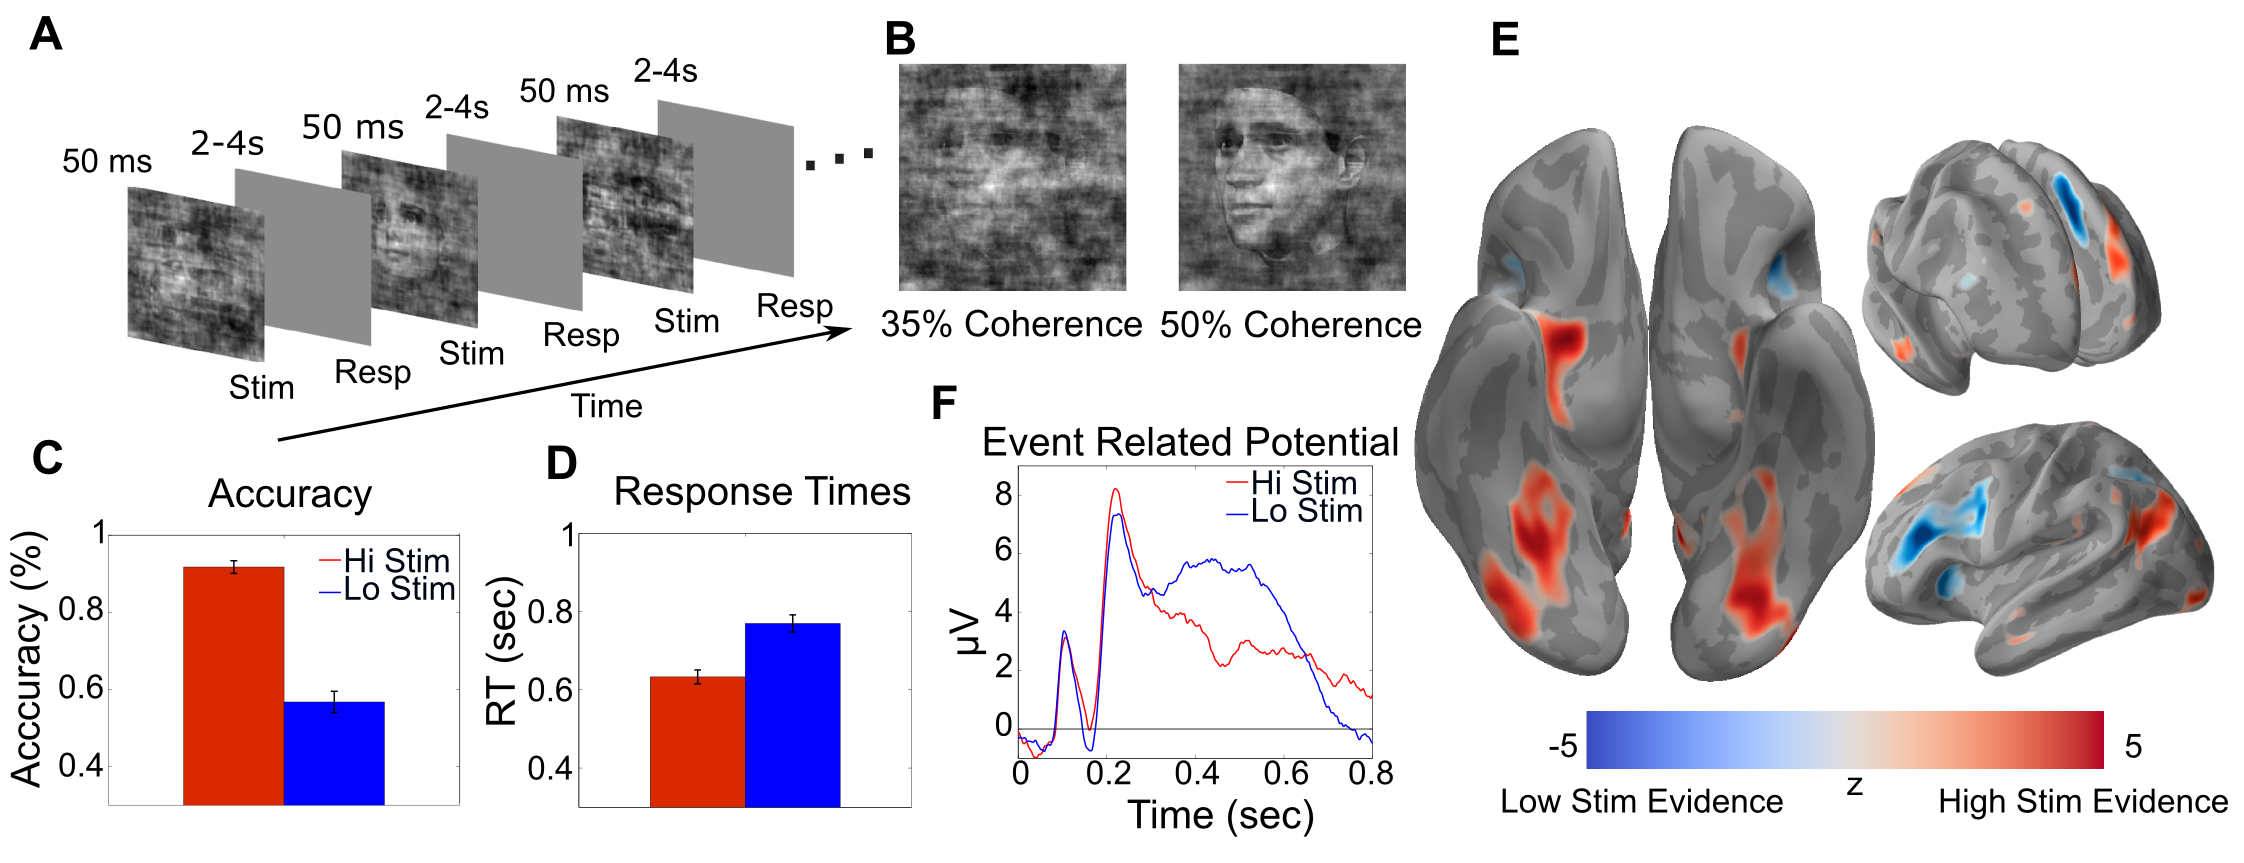
\includegraphics[width=1\textwidth]{Fig2.png}

\caption{ \textbf{Paradigm and traditional EEG and fMRI results.}\textbf{A}, 3-AFC task where stimulus evidence for each category is modulated by varying the phase coherence in the images. \textbf{B}, Example of face images with high stimulus evidence (high  coherence: 50\%) and low stimulus evidence (low coherence: 35\%). \textbf{C}, Behavioral performance shows significant differences, as a function of stimulus evidence, in accuracy ($p< 10^{12}$, paired t-test) and \textbf{D}, response time ($p< 10^{-8}$, paired t-test) across the group. \textbf{E}, fMRI analysis showing cortical areas correlated with high (red) vs. low (blue) stimulus evidence across the entire trial ($Z> 2.57$ with  $p< 0.01$ Family-Wise Error cluster corrected). \textbf{F}, Grand average stimulus-locked event related potentials (ERPs) for electrode Pz show that differences in stimulus evidence span the time from stimulus to response.}
\label{fig:TradResults}
\end{figure}
As a demonstration of how our method for encoding time-localized EEG variability in simultaneously acquired BOLD data can be used to infer neural cascades underlying perception and cognition, we collected EEG/fMRI data from subjects as they performed a 3-AFC task discriminating between faces, cars, and houses (Fig. \ref{fig:TradResults}A). Subjects were instructed to discriminate the object class after briefly viewing an image corrupted by varying levels of noise (Fig. \ref{fig:TradResults}B) and respond by pressing one of three buttons.  Overall, subjects responded with accuracies of 94 $\pm$ 5\% and 58 $\pm$ 12\% and with response times of 634 $\pm$ 82ms and 770 $\pm$ 99ms for high and low stimulus evidence trials, respectively (Fig. \ref{fig:TradResults}C, D). Subject accuracies and response times across stimulus types (faces, cars, houses) for low stimulus evidence trials were similar; however, for high stimulus-evidence trials subject accuracies were higher and response times were shorter for faces than for cars or houses (See Supplemental Information Fig. S1). 

\subsection*{GLM based analysis of BOLD fMRI shows superposition of cortical areas correlated with stimulus evidence}

We first used a traditional general linear model (GLM) analysis of the fMRI (see Methods) to demonstrate how a difference in stimulus evidence is reflected in in the BOLD data (Fig \ref{fig:TradResults}E, SI Table 1). These results become a baseline case we will compare to relative to the additional information that we can obtain using our encoding model for fusing the BOLD and EEG data. Brain regions showing greater BOLD activation to high vs. low stimulus evidence trials included areas associated with early visual perception and the default mode network, such as fusiform gyrus, parahippocampal gyrus, lateral occipital cortex, superior frontal gyrus, and posterior cingulate cortex. Regions with greater BOLD activation to low vs. high stimulus evidence trials included areas in the executive control and difficulty networks, such as dorsal lateral prefrontal cortex, anterior cingulate cortex, intraparietal sulcus, and insula. Important to note is that these GLM results, from simultaneous EEG and fMRI acquisitions, reproduced previous results in the literature for fMRI collected alone \cite{Heekeren2004}(Fig. S2A).  The encoding model results we present below are compared to these results in terms of how the temporal superposition of activations can be separated in time. 

\subsection*{Extracting temporally localized EEG signatures of stimulus evidence variability}

The traditional fMRI results showed multiple brain regions correlated with the stimulus evidence of the trial; however, this traditional approach does not enable one to infer the relative timing of these fMRI activations. However in the trial averaged event related potentials, we see that the difference in stimulus evidence (high vs. low stimulus evidence) spans the trial (see Fig \ref{fig:TradResults}F). To infer timing at a scale of tens of milliseconds, we exploit this difference and use linear classification \cite{Parra2005,Sajda2009} of the multichannel EEG to estimate EEG components selective to the trial-to-trial variability in the stimulus evidence.  Importantly these components were estimated at 25ms steps, locked to either the onset of the stimulus or response, so as to encode the BOLD activity at specified time points in the trial.  
\begin{figure}[tb!]
\centering
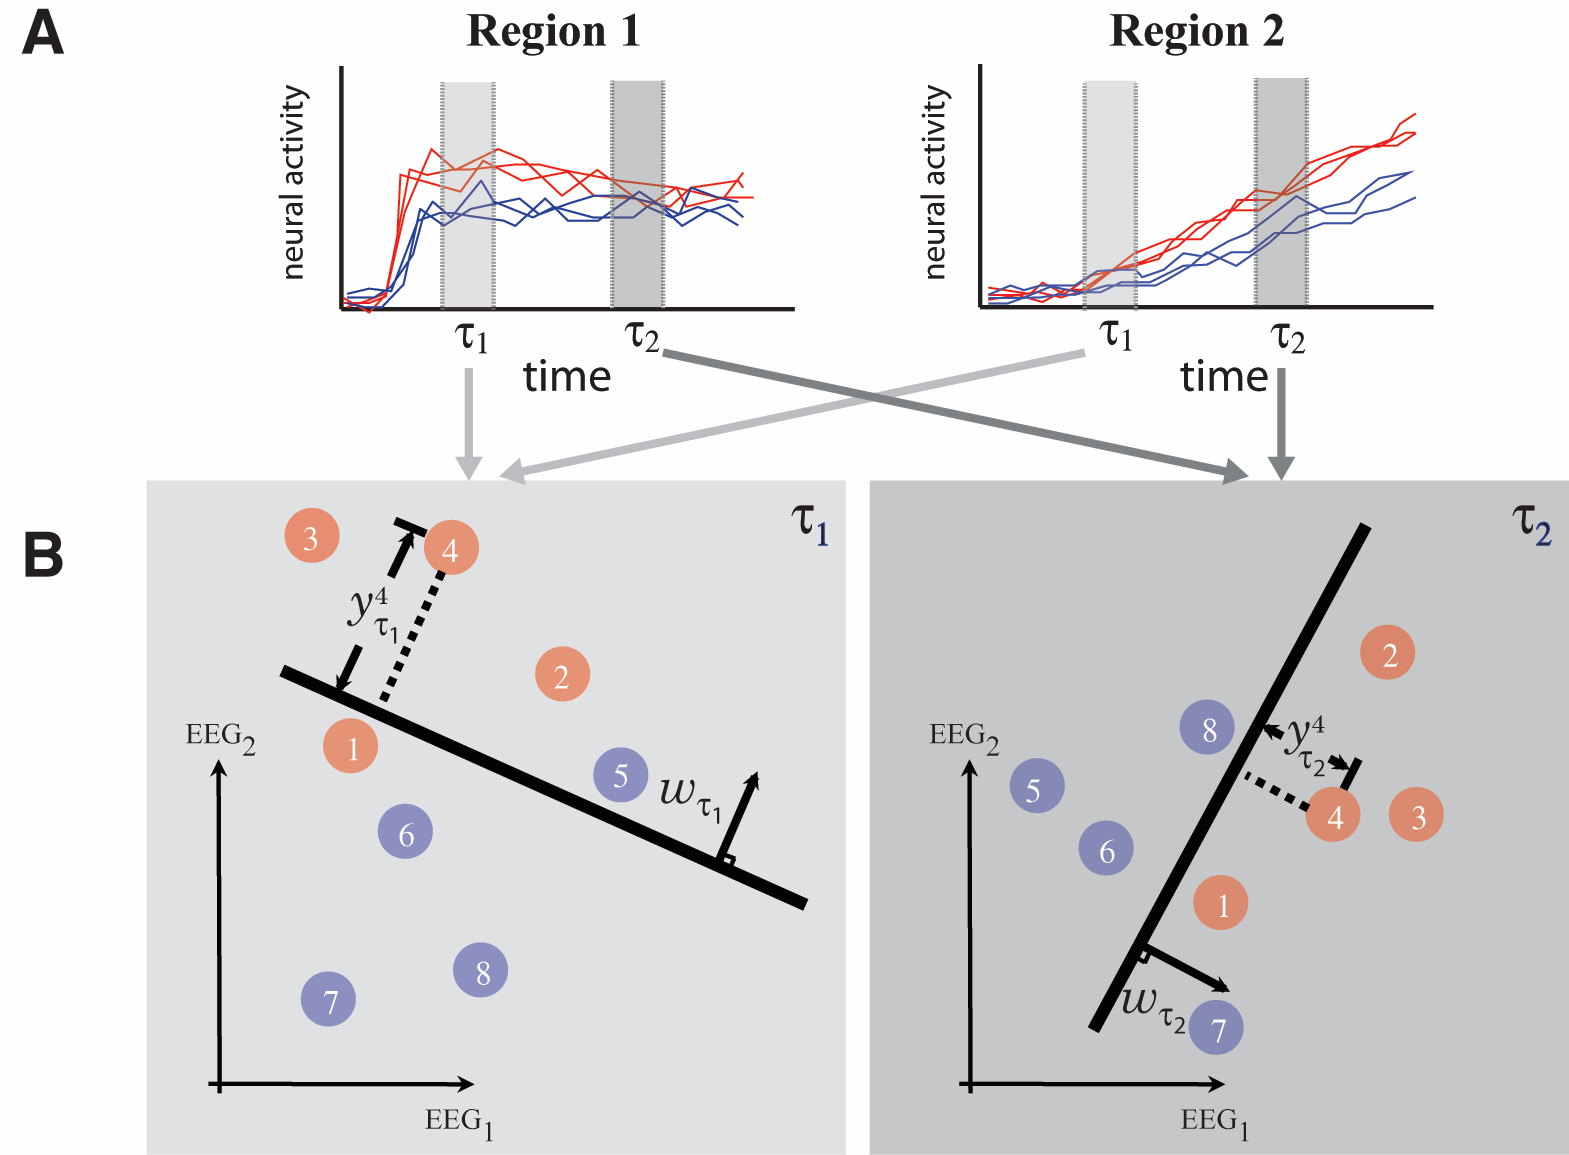
\includegraphics[width=.6\textwidth]{Fig3.png}
\caption{\textbf{Temporally precise trial-to-trial EEG variability tags brain regions during decision-making.}
\textbf{A}, Illustration of how trial-to-trial variability of neural activity in spatially distinct cortical areas can be used to tag brain regions. In this hypothetical example Region 1 is involved in sensory encoding while Region 2 integrates sensory evidence to form a decision (in NHP literature, Region 1 might represent MT, while Region 2 LIP). Neural activity across the trial is shown for two stimulus types, one with high sensory evidence for the choice (red curves) and one with low sensory evidence (blue curves).Also shown are two temporal windows ($\tau_{1}$ and $\tau_{2}$) that represent different times during the trial. \textbf{B}, Linear classifiers are trained to separate trials based on the two levels of stimulus evidence at specific temporal windows.  Shown are classifiers (parameterized by weight vectors $w_{1}$ and $w_{2}$) for two temporal windows ($\tau_{1}$ and $\tau_{2}$) with respect to two EEG sensors (for simplicity only two dimensions of the full N=43 sensor space are shown.  Though the component hyperplane is optimal for the full 43 dimensions, when projected to a line in two dimensions for illustration, it may appear that the separation is sub-optimal). This yields an EEG discriminant component for each temporal window. Variability along these components serves as a unique feature vector for temporally tagging the BOLD data—e.g. variability along an EEG component trained with data from $\tau_{1}$ tags BOLD voxels with time $\tau_{1}$ while variability along an EEG component trained with data from $\tau_{2}$ tags them with $\tau_{2}$.}
\label{fig:variability}
\end{figure}
The basic idea is illustrated in Figure \ref{fig:variability}, where hypothetical neural activity is shown for two different regions that are constituents of the perceptual decision-making network. Averaging over trials would clearly reveal a difference in the mean neural activity between high and low stimulus evidence (as we see in Fig \ref{fig:TradResults}F). However, the two regions contribute differentially to the network, with one region encoding the stimulus evidence (Region 1) and the other integrating it over time (Region 2); both are sensitive to the level of stimulus evidence, though varyingly so at different times in the trial.  By taking advantage of this sensitivity to the stimulus evidence, we can learn EEG discriminant components, i.e. spatial filters, that best classify trials at different time windows given the neural data.  We used the trial-to-trial variability along these component directions as features to uniquely tag fMRI voxels with the specific time window of the component. This tagging is done by building an encoding model of the features, given the BOLD signal, details of which are described in the following section.

We constructed EEG components by learning linear classifiers at 25ms steps, starting from stimulus onset to 50ms past the average low stimulus evidence response time. We chose a time step of 25ms due to an empirical analysis showing a half width of 50ms in the temporal autocorrelation of the EEG data, though in principle this methodology allows for temporal resolution up to the EEG sampling rate. Each classifier was associated with a set of discriminant values, which can be represented as a vector $y_{\tau}$; each element of the vector is the distance of a given trial to the discrimination boundary for the classifier at time step $\tau$ (Fig. \ref{fig:variability}). This distance can be interpreted as a measure of the EEG classifier's estimate of the level of stimulus evidence for that trial \cite{Goldman2009,Muraskin2015,Parra2005,Sajda2009,Sherwin2012,Walz2013}.

Results of the EEG analysis show discriminating information for stimulus evidence spanning the trial (see Fig. \ref{fig:EEGResults}A), beginning roughly 175ms post-stimulus to past the average response times.  A dip occurs around 300ms, indicating stimulus evidence is less discriminative at this time and serves to demarcate early and late cognitive processes. The early process corresponded to the time of the D220 ERP component, which has been shown to modulate with the degree of task difficulty, whether via stimulus noise or task demands \cite{Philiastides2006}. The later and more prolonged component is likely related to more complex cognitive and motor preparatory processes that differ between high and low stimulus evidence trials.  Importantly, although the early and late EEG components were both discriminative, we found their trial-to-trial variability to be uncorrelated (Figs. \ref{fig:EEGResults}B and S3E), indicating that while the discriminating information (level of stimulus evidence) persists across the trial, it couples differently to processes across time. 

\begin{figure}[h!]
\centering
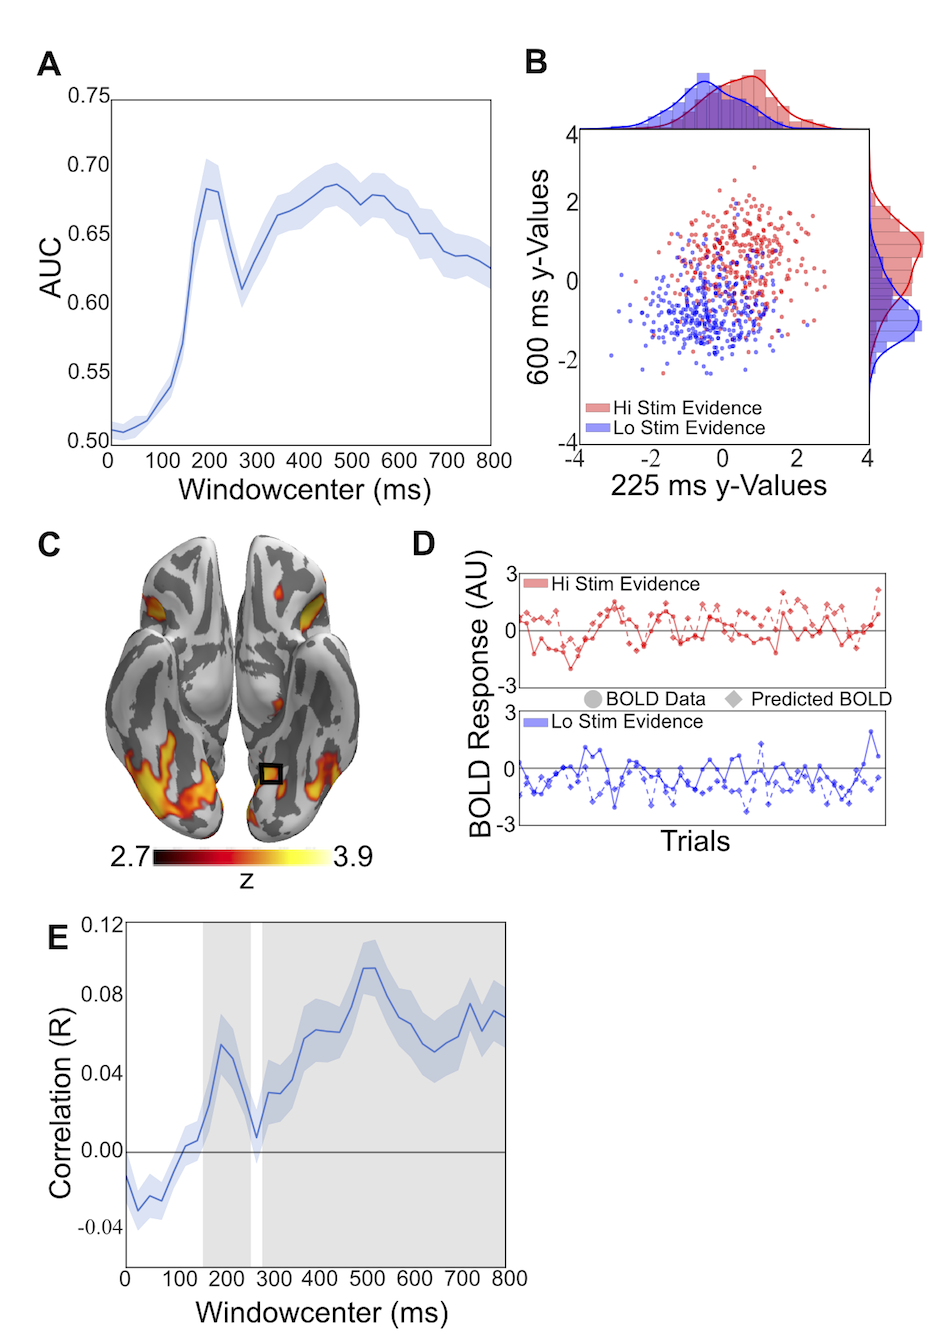
\includegraphics[width=.4\textwidth]{Fig4.png}

\caption{\textbf{EEG discrimination and encoding model results.}\textbf{A}, Group average area under the receiver operating curve (AUC) for the sliding window logistic regression EEG discrimination analysis, comparing high versus low stimulus evidence trials; standard error across subjects is shown with shading. \textbf{B}, A single subject's discriminating y-value distributions for high (red) and low stimulus evidence (blue) trials for two EEG time points (225ms and 600ms). \textbf{C}, Significant fMRI voxels resulting from the group level analysis for the encoding model ($p< 0.01$ TFCE-False Discovery Rate (FDR) corrected). Activity is seen encompassing early visual processing regions, attention networks, and the task positive network. \textbf{D}, A random subset of 100 (50 for each stimulus evidence condition) from 700 total trials of the actual (circle) and predicted (diamond) BOLD responses from the encoding model, for an example subject at a single voxel (MNI X/Y/Z mm: -27/-54/-15, r=0.206, $p<10^{-6}$). High and low stimulus evidence trials are shown separately for clarity. \textbf{E}, The averaged correlation of the predicted y-values with the true y-values across the trial duration. Blue shading represents the standard error across subjects. Grey shading indicates significant time windows ($p< 0.05$ FDR-corrected).}
\label{fig:EEGResults}
\end{figure}

\subsection*{Using an encoding model to link fMRI activations with temporally distinct EEG trial-to-trial variability}
After extracting the trial-to-trial variability from the EEG discriminant components, feature vectors $y_{\tau}$ are collected across time steps, $\tau$, along with a response time vector to construct a matrix $Y$. This matrix is the temporally precise representation of the trial-to-trial EEG variability that reflects high vs. low stimulus evidence. An encoding model (see Methods) is then fit to predict the trial-to-trial variability of the BOLD response for each fMRI voxel. The model can be seen as  ``taging" each voxel with a ``time", or set of times, when it encodes the variability in the given EEG discriminant component(s).

The group level result of the encoding model is shown in Fig. \ref{fig:EEGResults}C (see also Fig. S2B) where significant voxels from the encoding model are shown in yellow. Fig. \ref{fig:EEGResults}D shows the trial-to-trial variability of BOLD signal at a specific voxel, comparing it to the variability predicted by the encoding model. Additional validity of the encoding model and single subject results are presented in the Supplemental Information (Fig. S4A/B). The encoding model was also evaluated as a decoding model (see Methods) with the BOLD activity used to predict the trial-to-trial variability in the EEG for unseen data--data on which the encoding model was not trained. Fig. \ref{fig:EEGResults}E shows these results, expressed as the correlation between the measured and predicted EEG trial-to-trial variability across the 800ms epoch. The shape of the curve is highly consistent with that observed for the EEG data itself (comparing Fig. \ref{fig:EEGResults}A and Fig. \ref{fig:EEGResults}E) (additional analysis of the fidelity of the model is provided in the SI, Fig. S3).


\begin{figure}[htb!]
\centering
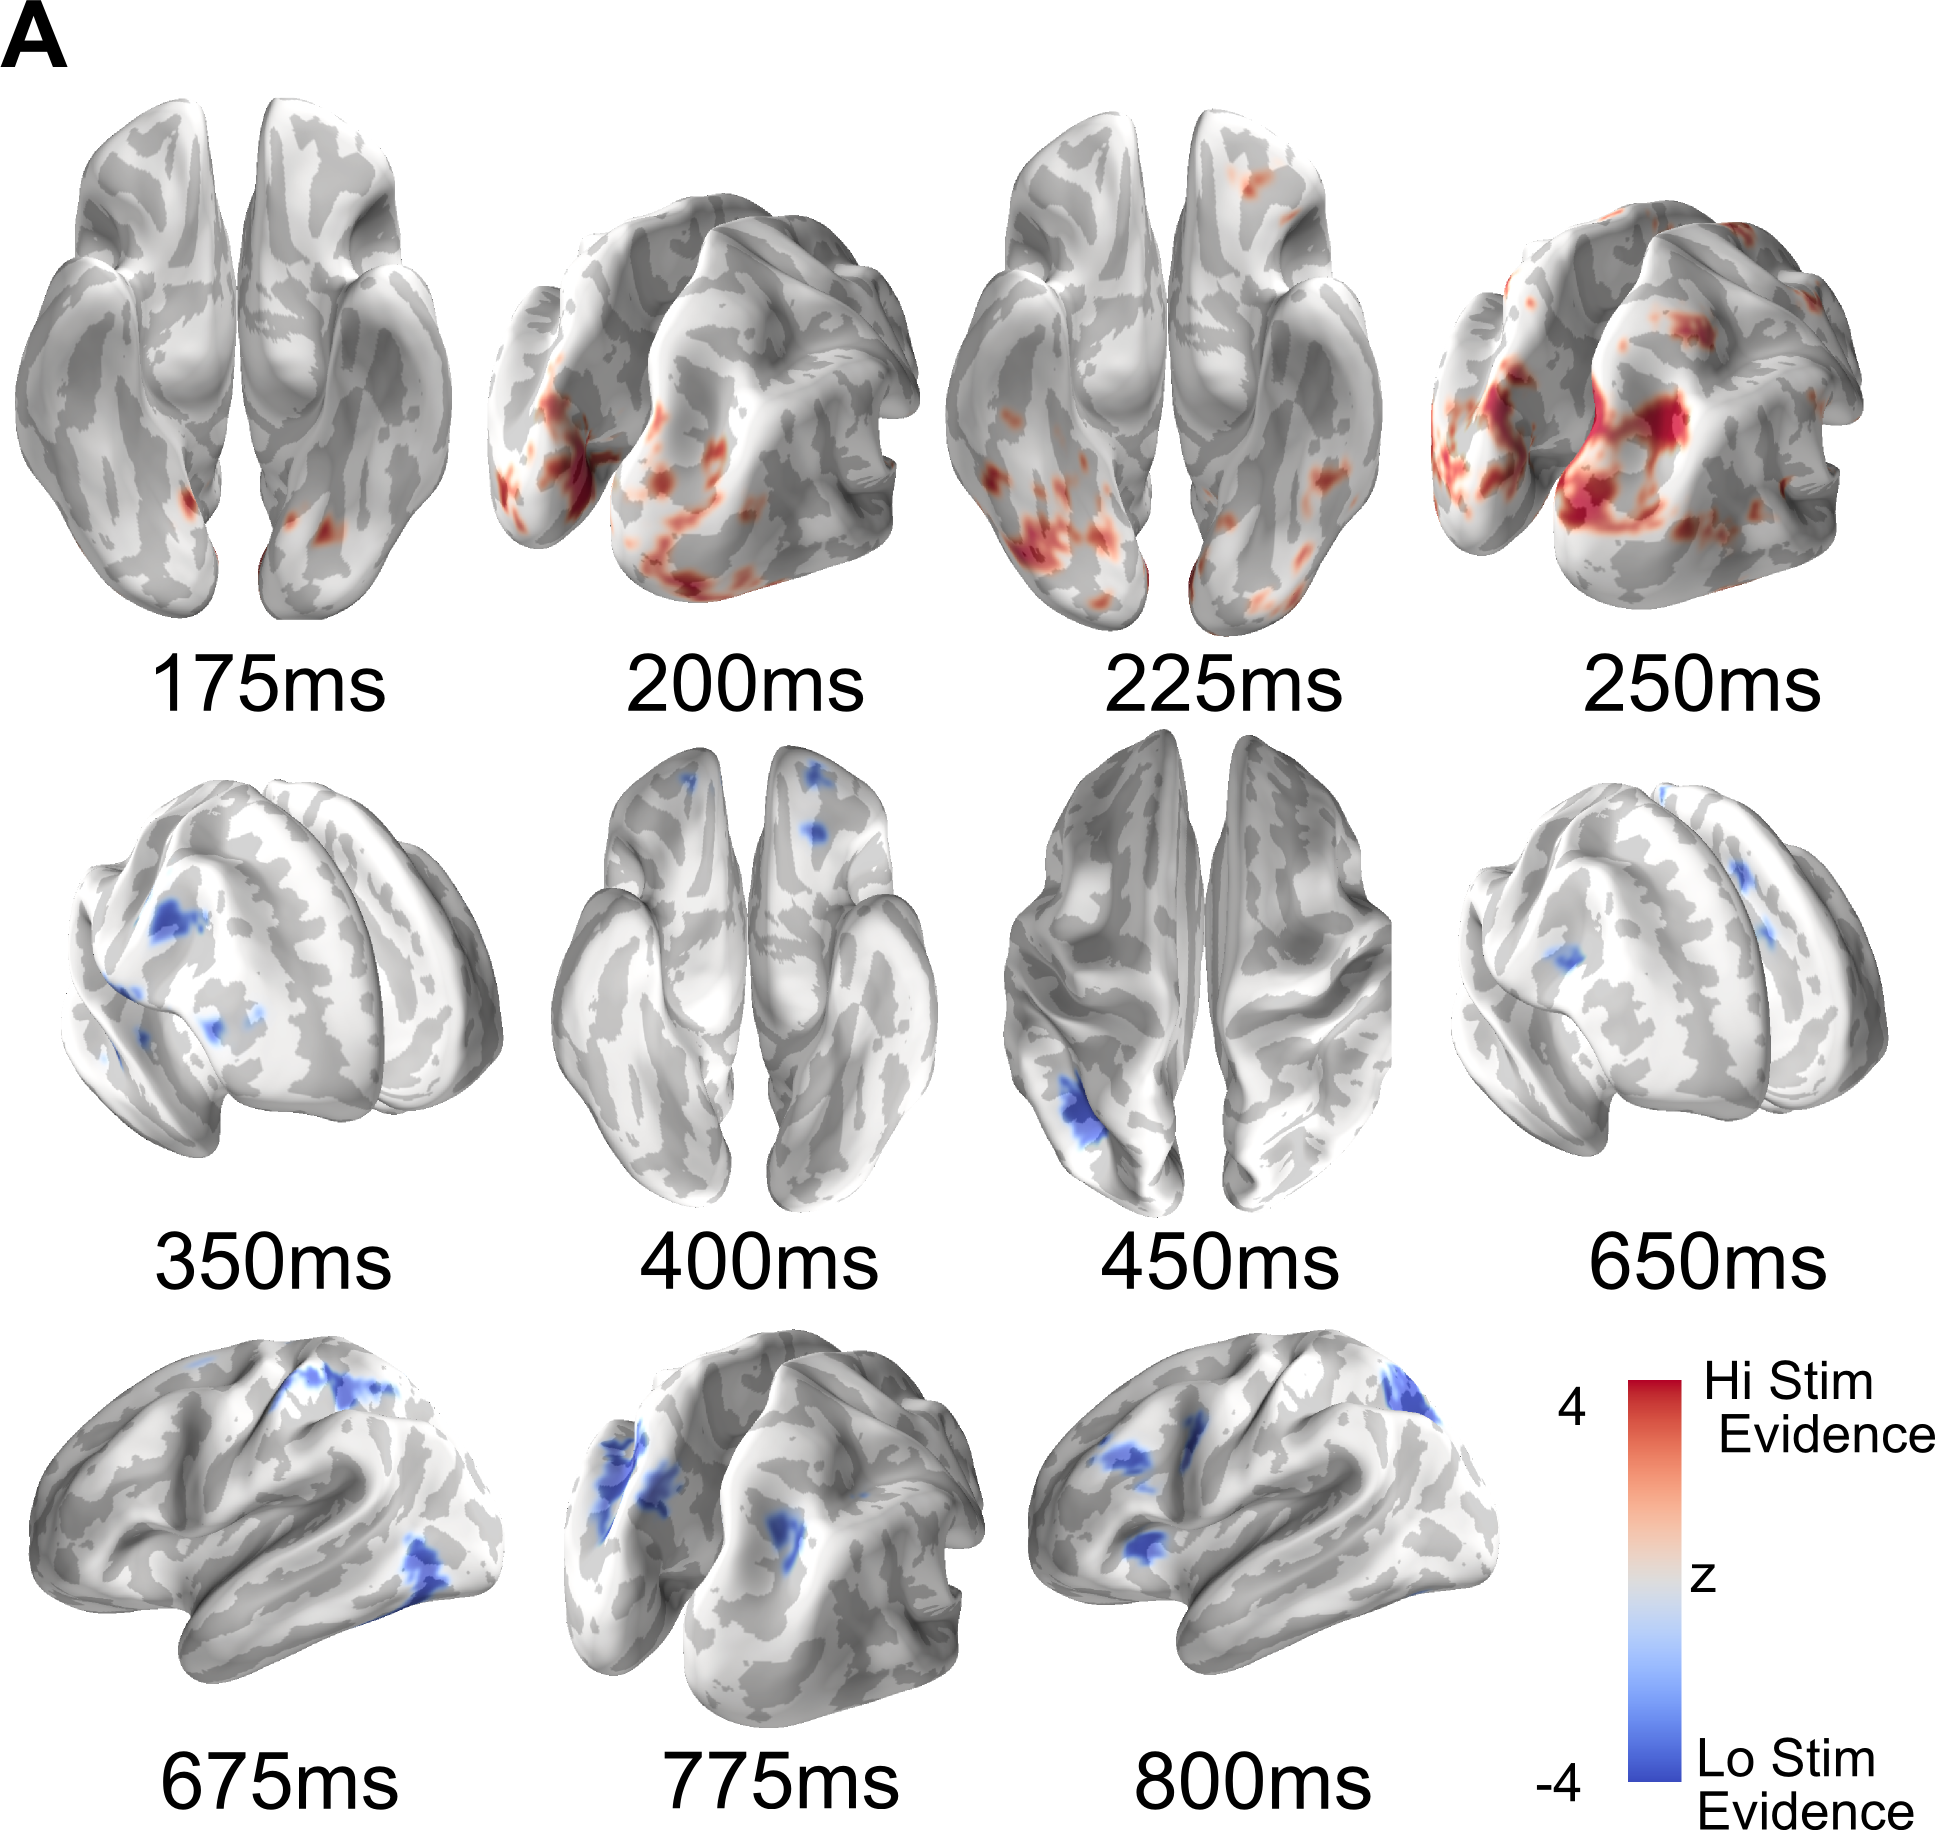
\includegraphics[width=.5\textwidth]{Fig5.png}
\caption{\textbf{Group-level encoding model weights results show neural activation cascade}. Subset of thresholded ($p< 0.05$ FDR-Corrected, k=10) group level statistical parametric maps created by stTFCE randomization procedure on the encoding model weight matrices show the progression of spatial activity across the trial. Activation can be seen early in the trial in the occipital regions while progressing more anteriorly later in the trial to executive control areas. Activations in red indicate areas where high stimulus evidence trials had larger activations than low stimulus evidence trials, and blue the inverse.}
\label{fig:fMRIResults}
\end{figure}

Given the encoding model, we construct the progression of the BOLD activity across time by identifying voxel weights that are consistent across subjects in space and time (see Methods). Fig. \ref{fig:fMRIResults} shows these results for a group level analysis. The weights from the encoding model can be interpreted similarly to the $\beta$-weights in a traditional GLM contrast. Here, red voxels indicate significant regions where high stimulus evidence variability positively covary between EEG discrimination y-values and BOLD activation and where blue voxels indicate a negative covariation between more negative EEG discrimination y-values (stronger low evidence discrimination) and BOLD activation. We observe a progression of activity (see also Movie S1), at 25ms resolution, which proceeds simultaneously down the dorsal and ventral streams of visual processing for the first 250ms. After that the cascade becomes more complex with activation in the IPS at 425ms and 750ms (see Fig. \ref{fig:EncodingResults}A), reactivation of the SPL at 675ms and activation of ACC at 600ms along with other regions found in the traditional fMRI results. (see Tables S2). The reactivation pattern is particularly significant since it would not be observable via a traditional fMRI general linear model (GLM) analysis (results of which were presented in Fig. \ref{fig:TradResults}E), which integrates over time and thus superimposes these activities. For example, the changing sign of the middle temporal gyrus (MT) encoding weights in Fig. \ref{fig:EncodingResults}A manifested as no activity in the MT for the traditional fMRI GLM analysis of this same BOLD data--the change in sign canceled the effective correlation in the GLM. The areas of activation we find are internally consistent with the traditional GLM results (see Fig. S2E/F) and with previous reports in the literature for human subjects \cite{Heekeren2004,Philiastides2007}; however, here we are able to link activations across time in a way that was previously only possible with invasive techniques. 

\begin{figure}[htb!]
\centering
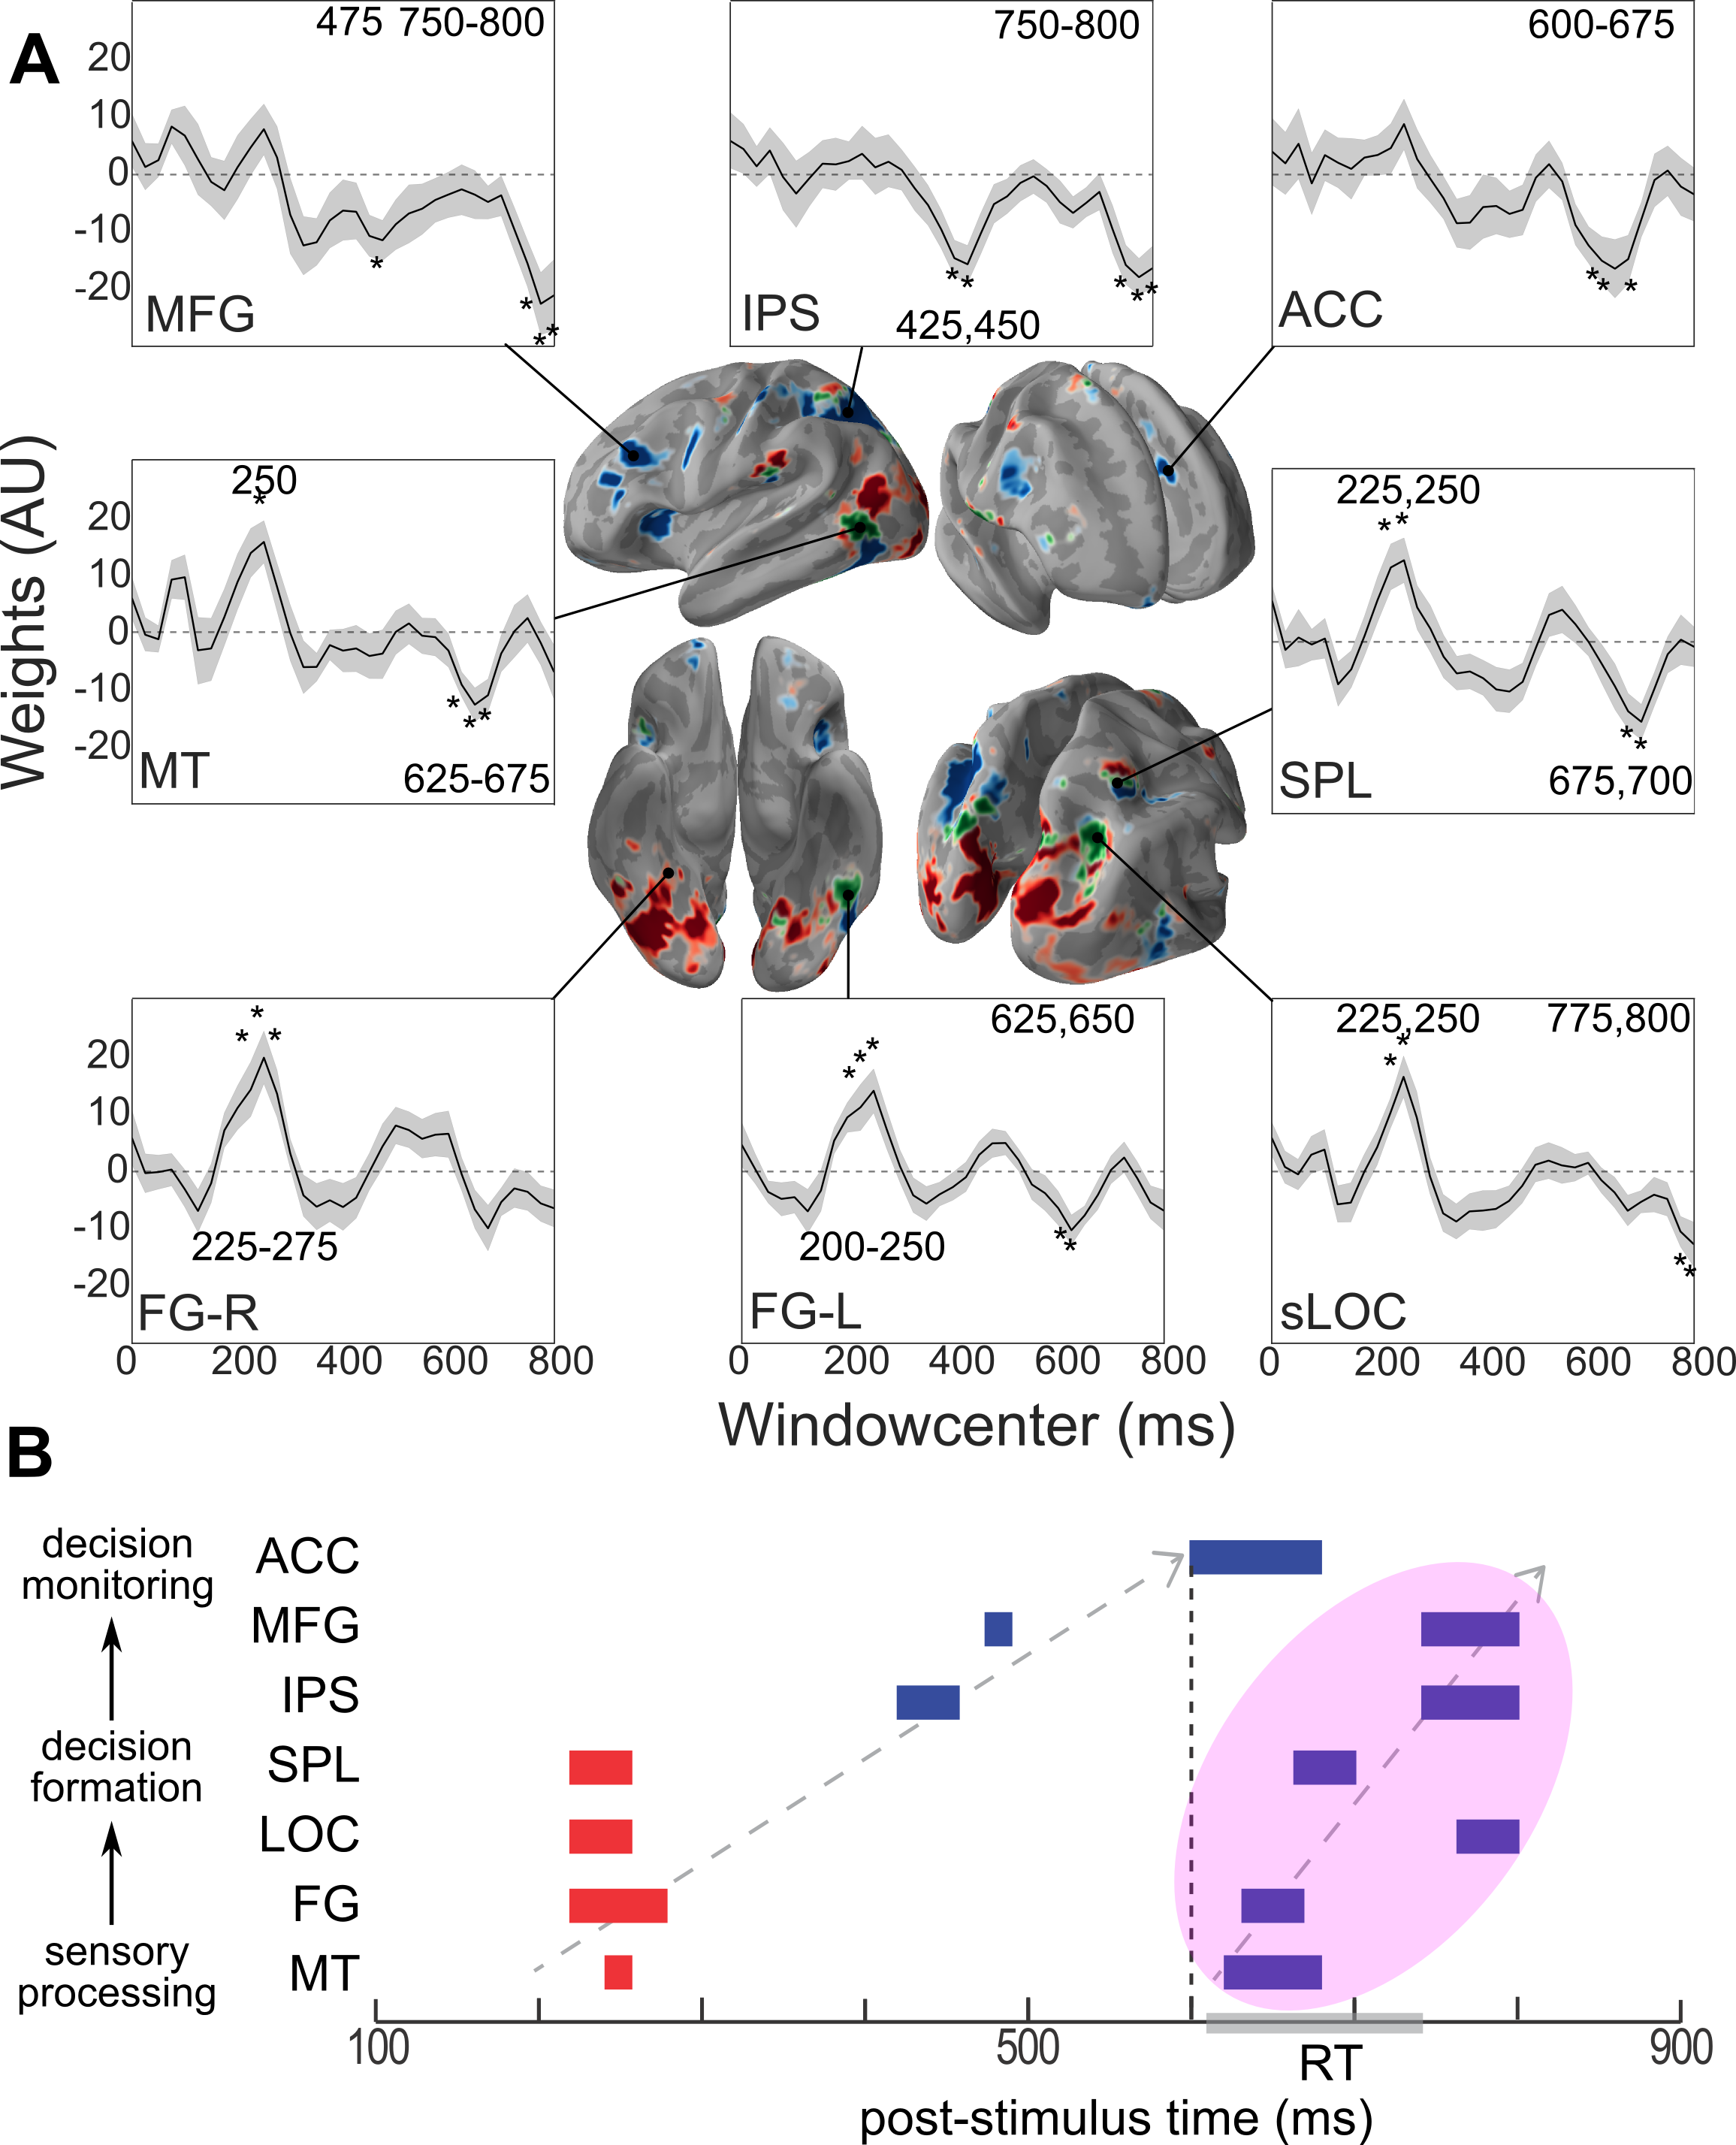
\includegraphics[width=.6\textwidth]{Fig6.png}
\caption{\textbf{Spatial-temporal event-related activations show coordinated reactivations.}\textbf{A}, Union across time windows of significant voxels for high (red) and low (blue) stimulus evidence activations. Voxels with activations for both high and low conditions (at different time windows) are displayed in green (Fig. S2C). Also shown are the encoding model weights for specific voxels, including fusiform gyrus (FG-R):36/-51/-18, (FG-L):-42/-42/-18, superior lateral occipital cortex (sLOC):24/-63/36, superior parietal lobule (SPL):27/-51/54, anterior cingulate cortex (ACC):-6/24/30, intraparietal sulcus (IPS):-30/-60/39, middle frontal gyrus (MFG):-45/27/30, middle temporal gyrus (MT):-57/-60/0. Asterisks indicate significant windows. \textbf{B}, Sequence of significant weights showing a ``replay" of the network after the onset of ACC activation (shaded ellipse). ``Replay" is faster than the initial stimulus driven sequence and strongest for low evidence trials.}
\label{fig:EncodingResults}
\end{figure}

\subsection*{Cortical reactivation correlates with decision confidence}

We identified a reactivation pattern in the spatiotemporal dynamics which was not observable using non-simultaneously acquired EEG or fMRI. Further analysis of the spatiotemporal dynamics (see Fig. \ref{fig:EncodingResults}B) shows that the reactivation pattern in the network occurs after decision-monitoring areas become engaged (i.e. after activation of ACC).

Spontaneous reactivation, or ``replay," of neural activity in the human brain has been observed and is believed to be important for memory consolidation \cite{Deuker2013} and more recently has been hypothesized to play a role in perceptual decision-making by enabling the formation of decision confidence \cite{Fleming2012}. To test the hypothesis that the reactivation activity we see may be related to decision confidence, we used a hierarchical drift diffusion model (DDM) \cite{Ratcliff2008,Wiecki2013} to fit the behavioral data for high and low stimulus evidence conditions (see Methods).  Specifically, our model enables us to define a proxy for decision confidence based on the DDM fits to the behavior \cite{Kiani2014,Philiastides2014}. 

Correlating the reactivation level to this confidence proxy shows a strong and significant monotonic relationship between confidence proxy and the level of reactivation (high stimulus evidence-slope=0.037$\pm$0.008, t=4.657, $p=3.2x10^{-6}$; low stimulus evidence-slope=0.062$\pm$0.008, t=7.754, $p=8.88x10^{-15}$), with low stimulus evidence trials reactivated more strongly than high stimulus evidence trials (difference in slopes=-0.025$\pm$0.011, t=2.189, p=0.029)(see Fig. \ref{fig:Confidence} and Fig. S5a). Additionally, reactivation amplitude correlates with behavioral accuracy (Fig. S5b) (high stimulus evidence, slope=0.0115$\pm$0.0047, t=2.41, p=0.016; low stimulus evidence, slope=0.0104$\pm$0.0047, t=2.19, p=0.028).  Additional control analyses from early time windows (175-250ms) shows no significant correlations between activation and confidence proxy (Fig. S5).

We next analyzed which cortical regions most contributed to this reactivation. Specifically, we used a recursive feature elimination to identify those regions contributing the most to the correlation between the level of reactivation and the confidence proxy.  We found that the IPS/SPL and dorsal lateral prefrontal cortex (DLPFC) contributed the most (Fig. \ref{fig:Confidence}C). Interestingly, these two areas have been previously implicated in metacognitive judgments of confidence \cite{Fleming2012,Steinhauser2010,Yeung2012}.

\begin{figure}[htb!]
\centering
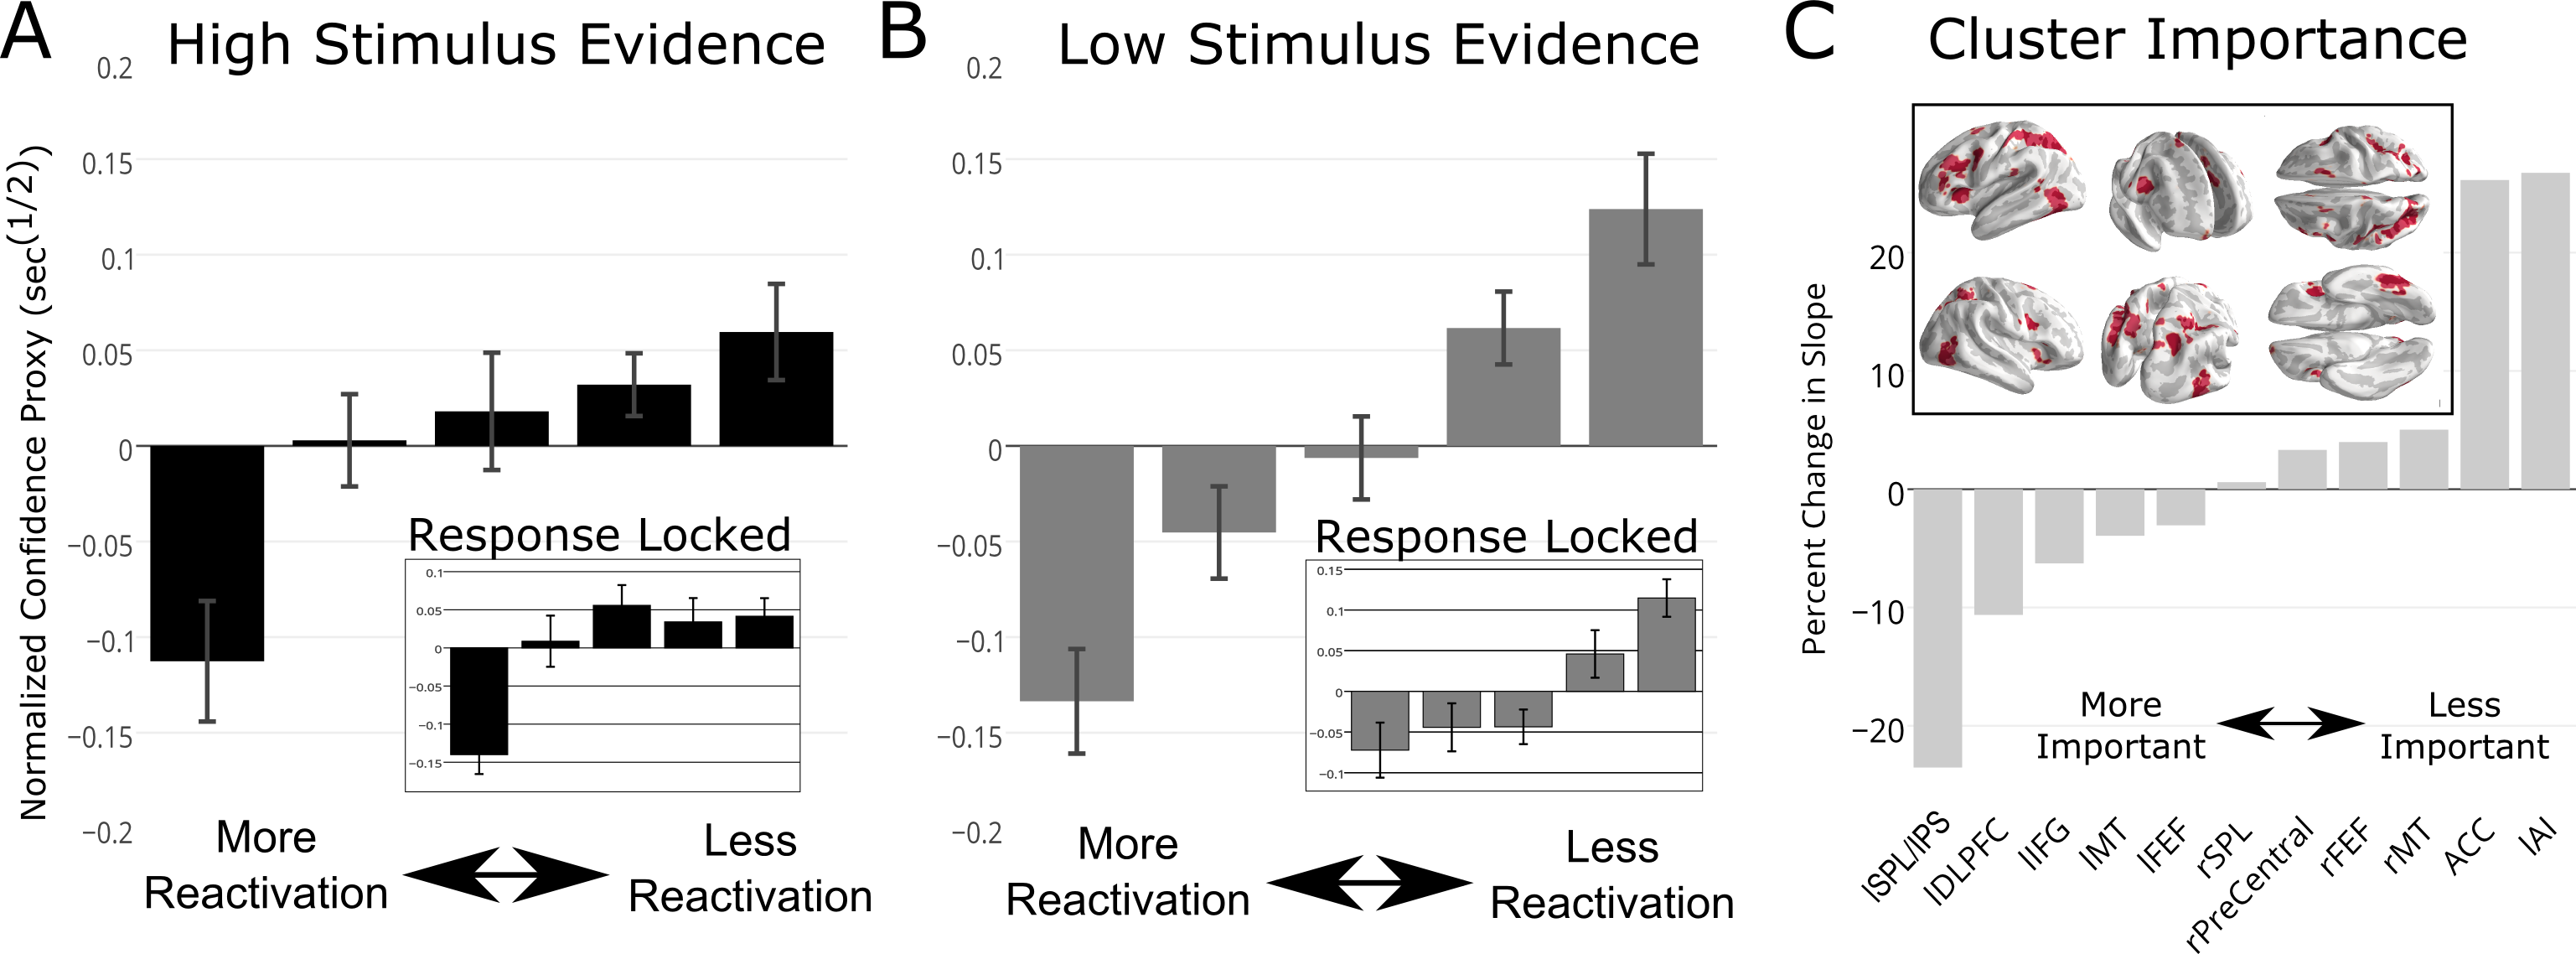
\includegraphics[width=1\textwidth]{Fig7.png}
\caption{\textbf{Trial-to-trial reactivation correlates with decision confidence.}Trial-to-trial reactivation amplitude ($Y^{R}_{j,i}$ – see Methods) of ``replay" correlates with confidence proxy for both high (\textbf{A}) and low (\textbf{B}) stimulus evidence conditions. Error bars represent standard errors across subjects. Response locked analysis results are shown in the insets for (\textbf{A}) and (\textbf{B}) as well as Fig. S6-7. \textbf{C}, Stimulus-locked replay activation clusters and feature importance. (inset) Regions of interest used in computing the reactivation values for computing confidence proxy correlations. These regions were taken from significant group activations from 600-800ms post stimulus.  Regions were then clustered ($> 48$ voxels) and a secondary analysis for feature importance was performed. Here, we removed each cluster before computing trial-to-trial reactivations and compared the slope of reactivation x confidence proxy when all clusters were present.  Panel \textbf{C} shows the ranking of feature importance for each cluster (more negative \% change = more importance). Negative changes in slopes indicate that by removing that cluster the slope of the correlation between reactivation and confidence decreases indicating the importance of that cluster.}
\label{fig:Confidence}
\end{figure}